\documentclass[11pt]{article}

\usepackage{fullpage}
\usepackage{graphicx}
\usepackage{hyperref}
\usepackage{array}

\title{Comparing Backoff \& Ensemble Strategies for Latin Text Lemmatization}
\author{Janaki Mohta}
\date{07-28-2025} %don't display the current date

\begin{document}

\maketitle

\begin{abstract}

Lemmatization is a vital first step in Latin natural language processing, which enables further computational analysis of Latin texts. This project tests and compares the capabilities and algorithmic strategies of the Classical Language Toolkit library’s lemmatizers and their components. In particular, it examines the Backoff strategy of lemmatization and compares it with the Ensemble method, which was promising but less prevalent than expected. I ultimately found that the CLTK Backoff sub-lemmatizers were highly specialized and thus did not perform as well in an Ensemble configuration. However, the findings open prospects for further experimentation with Ensemble across larger groups of lemmatizers more similar to one another. In particular, implementation of Ensemble could be a low-effort point of improvement for strong modern lemmatizers.
  
\end{abstract}

\section{Introduction}
In natural language processing, an important first step is to reduce tokens (units of meaning, typically a single word or punctuation mark) into simpler forms. For many languages, including English, one solution is stemming, removing prefixes and suffixes to get a token’s base form (Manning et al., 2009) \cite{info_retrieval}. This system tends to be simple and often imprecise, but it is efficient. However, in some languages, simple stemming algorithms are no longer effective, largely due to the languages’ morphological complexity, having many forms of each word and similar forms between different kinds of words (Popovi\v{c} and Willett, 1992) \cite{stemming_effectiveness}. Instead, better results can be obtained through a method called lemmatization. Algorithms, called lemmatizers, analyze each token and output a lemma, a predetermined standardized form of the token (Sprugnoli et al., 2020) \cite{sprugnoli_lemmatization}. They employ a wide variety of different methods, and in many models, a group of sub-lemmatizers is assembled into a larger lemmatizer. This project focuses on two possible methods for organizing sub-lemmatizer groups: a system called Backoff (NLTK Project, 2024; Burns, 2018) and another called Ensemble (Burns, 2019; Burns, 2020) \cite{nltk_proj} \cite{philological} \cite{multiplex} \cite{ensemble}. Backoff employs one lemmatizer at a time in a chain, while Ensemble uses all the lemmatizers at once and returns the most frequent output between them. I chose to focus on Latin because it has enough morphological complexity to pose a challenge, while also having a relatively large and well-maintained corpus. In order to test these strategies, I employed a Github library called the Classical Language Toolkit (CLTK; Johnson et al., 2021), which offers lemmatization tools for many Classical languages, including Latin \cite{johnson-etal-2021-classical}. While not as powerful as more recent tools like Stanza (Stanford NLP Group, 2023) and LatinCy (Burns, 2023), CLTK provides a simpler arena for assessing the benefits of Backoff and Ensemble lemmatization \cite{stanford_nlp_stanza} \cite{latincy}. These tools, if proven successful, could then be applied to improve more complex lemmatizers. 

This project tests each CLTK sub-lemmatizer individually and experiments with creating custom Backoff lemmatization pipelines. It also explores the CLTK Ensemble lemmatization system, developed as a result of a promising paper by Patrick Burns (2020)\cite{ensemble}. However, while the paper focused on using Ensemble between multiple complete lemmatizers, the CLTK implementation instead provided infrastructure for an Ensemble system using Backoff components. I was interested to compare the two. I was also surprised that after initial positive reception, the system had lapsed in popularity, to the extent that the CLTK Ensemble Lemmatizer had been removed from the project’s repository. I wanted to understand why its usage remained narrow and to test its continued utility in order to better understand what tools are most effective for Latin lemmatization more broadly. Using Julius Caesar's \textit{Comentarii De Bello Gallico}, Book 1, Chapter 1, I collected and analyzed data on the accuracy of the various lemmatizers and pipelines.


\section{Background}

Lemmatization involves taking a token and reducing it into its base form. For example, the  English tokens “running” and “ran” would both be lemmatized into the token “run.” In Latin, the words “cursurus” and “currere” would both be lemmatized into “curro,” the first person singular form of the verb. As shown in these examples, lemmatization can normalize tokens despite a variety of grammar constructions, even those that change the tokens’ part of speech. “Running” in English and “cursurus” in Latin are both participles, adjective forms of a verb, but lemmatization still returns them to their verbal base form.

One leading strategy for lemmatization is a Backoff lemmatizer, in which multiple sub-lemmatizers are employed in a chain. Given a token, the pipeline's first sub-lemmatizer attempts to find a lemma match. If it can, the system continues to the next token. Otherwise, the next sub-lemmatizer attempts to find a lemma. The process continues until every token has a lemma.

CLTK's Latin Backoff lemmatizer employs a backoff system with five different types of lemmatizers: 

\begin{enumerate}
  \item The Dict lemmatizer consults a dictionary to find an exact match for the token (OpenNLP Documentation, 2017) \cite{apache-opennlp}. \\ \\
For example, given the input “templi” into the Dict lemmatizer, it would search for an exact entry in its dictionary matching “templi” to its lemmatized form “templum. If it found “templo”  or “templa,” it would not be able to draw the connection to “templi.” 

  \item The Unigram lemmatizer, based on NLTK’s Ngram taggers, assigns a lemma based on a corpus of training data (Bird et al., 2009) \cite{bird-et-al}. \\ \\
Given the input “templi” into the Unigram lemmatizer, it might use its training data to observe that “templo,” “templa,” and “templis” all lemmatize to “templum” and thus conclude that “templi” lemmatizes to “templum” as well.

  \item The Regexp lemmatizer is essentially a stemmer, using a list of standard word endings to remove potential stems and replace them with the word’s standard form (NLTK Documentation, 2024) \cite{nltk_proj}. \\ \\

  With the input “templi,” the Regexp lemmatizer might have a reference that the standard form of the ending “-i” could be the ending “-um.” However, in Latin there are multiple word forms that could end in “-i,” creating a potential source of error for Regexp. For example, since the Latin word “equus” can take the form “equi,” Regexp could employ the “us”/”i” pattern to incorrectly lemmatize “templi” as “templus.”


  \item The Identity lemmatizer returns exactly what was input (Burns, 2018) \cite{philological}. \\ \\
  If “templi” were inputted into the Identity lemmatizer, “templi” would also be the output. This, of course, would be incorrect. The Identity lemmatizer functions as a backup: for any token, there is some chance that it is in its base form, which would result in a correct output.

\end{enumerate}

In CLTK’s Backoff lemmatization pipeline, the first lemmatizer is a Dict lemmatizer referencing the CLTK “latin\_model” dictionary, which has just 689 entries. Then, the Unigram lemmatizer searches for lemmas. The Regexp lemmatizer then stems some of the remaining unlemmatized tokens using CLTK’s built-in list of common word endings, “latin\_sub\_patterns.” Next is an older version of the Dict lemmatizer, which consults the “latin\_lemmata\_cltk” dictionary and will be referred to as Old Dict. Old Dict’s dictionary is much larger than Dict’s, with 270,227 entries, and contains 563 of the items in Dict’s dictionary. Finally, the Identity lemmatizer ensures that every token has a lemma.

In the Ensemble lemmatizer, rather than “backing off” in a chain, each lemmatizer functions separately and returns a set of lemmas weighted by confidence. Then, the lemma with the highest cumulative weight is output. The CLTK Ensemble system allows usage of Unigram, Dict, and Regexp lemmatization. I was curious as to why Identity was not included and tried to implement it; I found that since the Identity Lemmatizer is a final measure, designed to always return a lemma rather than to be accurate, its outputs tended to skew the results. 

\section{Methods}

Except with Ensemble, as noted below, this project used CLTK 1.5.0, in a virtual environment running Python 3.9.23, as it was the most recent Python version supported by CLTK.

The CLTK sub-lemmatizers are packaged into the Backoff pipeline. I created individual instances of each sub-lemmatizer, trained on the same data as in the Backoff chain. To ensure that each lemmatizer had been created correctly, I assembled a custom pipeline with my versions of the sub-lemmatizers, called “backoff\_clone.” The clone’s outputs were identical to the Backoff lemmatizer’s, a sign that the sub-lemmatizers had been accurately isolated.

Next, I ran tests on the different sub-lemmatizers, analyzing how they lemmatized their inputs, their strengths and weaknesses, and their overall performances. To start, I used a variety of different Classical Latin authors and texts: Caesar’s \textit{Commentarii De Bello Gallico} and Cicero’s first Catilinarian Oration, both written in prose, and Virgil’s \textit{Aeneid}, a poetic text. The three texts were well-known, easily processable, and generally considered good representation of their genres. After noticing avoidable errors in the lemmatization, I implemented some of CLTK’s text processing functions on my text dataset: the “remove\_que” function, which removes the “-que” suffix, and the “replace\_jv” function, which standardizes v’s and j’s into u’s and i’s. In Latin, the suffix “que” corresponds to the English word “and,” and is a distinct token despite being attached to another word. Also, classical Latin did not distinguish between J and I or between U and V. The extra letters were introduced to Latin later, and as a result, they can lack standardization, which can interfere with lemmatization. It became clear that similar irregularities occurred more often in poetic texts than prose ones. Given the limited scope of the project, I decided to focus on prose to assess the lemmatizers in a more standardized linguistic environment.

Partly due to unusually high performance with the Catilinarian Oration (I later discovered that Unigram's training data included the exact excerpt I used), I decided to focus on \textit{De Bello Gallico} and created a dataemmatizers how it did, and whether its order could be optimized. In
particular, I was interested to establish a quantitative pattern for the order of the lemmatizers in
the Backoff chain.
I also ran similar tests on the Ensemble lemmatizer. The code had been removed from the most
recent version of CLTK, so I dset of lemmatized tokens from Book 1, Chapter 1 of the text. I occasionally consulted the Whitaker’s WORDS lemmatizer (Keegan), a tool with a large reference library and thus fairly high accuracy, to assist with lemmatization when unsure of a lemma \cite{whitakers-words}.

Next, I tested the lemmatizers on random slices of increasing sizes from the 211 tokens, establishing that performance was consistent between the sample sizes and thus that my small dataset would still represent the lemmatizers’ overall accuracy with \textit{De Bello Gallico}. However, the smoothing effect over time could be somewhat misleading, as the small data size led to likely overlap between the different slices. If one slice included some of the same tokens as the previous slice, its accuracy would be unnaturally similar to the previous data point. This problem would increase in severity as the sample sizes grew larger, since there are fewer possible large slices than small slices.

\begin{figure}
    \centering
    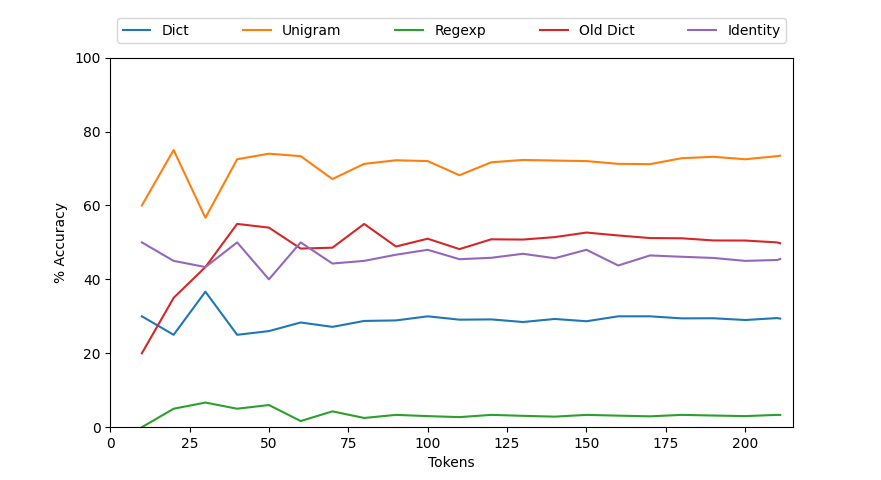
\includegraphics[width=0.5\linewidth]{accuracy_over_time_v3.png}
    \caption{Accuracy of each sub-lemmatizer with varying amounts of tokens.}
    \label{fig:enter-label}
\end{figure}

Once I had obtained and processed the data about the individual lemmatizers, I ran them in groups, creating custom Backoff pipelines. The custom pipelines allowed me to analyze why CLTK’s Backoff pipeline ordered the lemmatizers how it did, and whether its order could be optimized. In particular, I was interested to establish a quantitative pattern for the order of the lemmatizers in the Backoff chain.

I also ran similar tests on the Ensemble lemmatizer. The code had been removed from the most recent version of CLTK, so I downloaded it from a previous version of the library (Burns 2020) \cite{ensemble_add_burns_2020}. As mentioned above, the Ensemble lemmatizer class contains three lemmatizer tools: the Ensemble Regexp lemmatizer, the Ensemble Dict lemmatizer, and the Ensemble Unigram lemmatizer. I created one Ensemble sub-lemmatizer for each of the CLTK Backoff sub-lemmatizers. I also stripped extraneous numbers from the lemmatizations, as lemmas like “incolo1” were counted as separate from “incolo,” disrupting the weighting. Then, I organized these lemmatizers in custom groups and analyzed their outputs.

\section{Results}

First, I observed the performances of the individual sub-lemmatizers to understand their roles in the Backoff chain. I had initially assumed that the ordering of the lemmatizers would relate to the error rates of each lemmatizer, with less-frequently incorrect lemmatizers positioned earlier in the chain. However, I was surprised to notice that the Regexp lemmatizer, positioned after the Unigram lemmatizer in the chain, had a much lower raw error rate. 

\begin{figure}
    \centering
    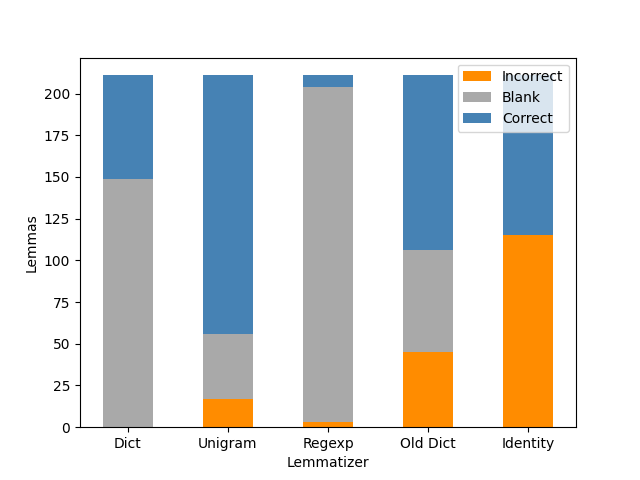
\includegraphics[width=0.5\linewidth]{sub_lemmatizer_performance.png}
    \caption{Performances of the individual sub-lemmatizers.}
    \label{fig:enter-label}
\end{figure}

In fact, instead of error rate, these tests revealed that CLTK Backoff chain’s order is related to the ratio of correct to incorrect lemmas, which will be referred to as the accuracy ratio.


    \begin{table}[]
        \centering
        \begin{tabular}{| c | c |}
             \hline
             Sub-Lemmatizer & Accuracy Ratio \\
             \hline
             Dict & inf. \\
             Unigram & 9.12 \\
             Regexp & 2.33 \\
             Old Dict & 2.33 \\
             Identity & 0.835 \\
             \hline
        \end{tabular}
        \caption{Ratio of correct to incorrect lemmas (ignoring blanks) for each sub-lemmatizer.}
        \label{tab:my_label}
    \end{table}

The lemmatizer at the start of the chain, Dict, returned no incorrect lemmas in this test and had an infinitely high accuracy ratio. It leaves many tokens blank but returns almost entirely correct lemmas, making small but high-accuracy progress on the unlemmatized list of tokens.

The second lemmatizer, Unigram, also has a relatively high accuracy ratio. Its placement as second in the CLTK Backoff chain gives it precedence to lemmatize the majority of the tokens with relatively high accuracy. While it is not perfect, and also does not always return a lemma, its well-roundedness makes it effective as the second lemmatizer.

The next lemmatizer, Regexp, has a substantially lower accuracy ratio of 2.33, returning just over two correct lemmas for each incorrect one. Despite its low raw error rate, as mentioned above, its low accuracy ratio prevents it from going earlier in the chain.

The main role of the next lemmatizer, Old Dict, is to fill in gaps left by the previous lemmatizers. It has the same accuracy ratio as Regexp, but its higher raw error rate places it second between the two.

Finally, the Identity lemmatizer ensures that every token has a lemma. Its accuracy rate is 0.835, the lowest of the group but still reasonably high. Interestingly, the ratio is close to 1, indicating that just under half of tokens are already in their lemmatized form.

Thus, the CLTK Backoff chain organization can be viewed quantitatively as a gradient from high to low correct-incorrect lemma ratios. It is also important to note that in practice, lemmatizers with higher accuracy rates tend to avoid incorrect answers by leaving more lemmas blank, which leads to the general trend of decreasing amounts of blank outputs. This is useful for assembling a Backoff chain, since earlier lemmatizers can leave more blanks than later ones.

I was interested to see whether rearranging the sub-lemmatizers by other metrics would produce stronger results than the standard Backoff pipeline. Experimenting with custom Backoff chains, I found that the CLTK Backoff pipeline consistently performed better than any other combination of its components, including when they were reordered by error rate. A variety of custom pipeline configurations achieved an accuracy of above 80\%, but none approached or exceeded the 85\% accuracy of CLTK’s pipeline.

    \begin{table}[]
        \centering
        \begin{tabular}{| p{0.5\linewidth} | c |}
             \hline
             Pipeline & Accuracy \\
             \hline
             CLTK Backoff & 0.853 \\
             CLTK Backoff without Dict & 0.839 \\
             Min Error \newline (Dict, Regexp, Unigram, Old Dict, Identity) & 2.33 \\
             Old Dict \newline (Unigram, Old Dict, Identity) & 2.33 \\
             \hline
        \end{tabular}
        \caption{Ratio of correct to incorrect lemmas (ignoring blanks) for each sub-lemmatizer.}
        \label{tab:my_label}
    \end{table}

These results demonstrate the extent to which the Backoff lemmatizers are optimized for their roles. Each component is strategically placed by accuracy ratio, as described above, and any reordering results in a worse configuration of the same relatively strong components. The custom pipelines that least adjusted the standard pipeline order tended to perform best, indicating that CLTK Backoff is heavily specialized for its standard order.

Similarly, I analyzed whether any Ensemble lemmatizers could approach the accuracy of CLTK Backoff.

    \begin{table}[]
        \centering
        \begin{tabular}{| c | c | c |}
             \hline
             \ & Components & Accuracy \\
             \hline
             \  & CLTK Backoff & 0.853 \\
             A & Old Dict, Dict, Unigram, Regexp & 0.796 \\
             B & Old Dict, Unigram, Regexp & 0.796 \\
             C & Old Dict, Dict, Unigram & 0.777 \\
             D & Old Dict, Unigram & 0.777 \\
             E & Dict, Unigram, Regexp & 0.763 \\
             \hline
        \end{tabular}
        \caption{Comparing the accuracies of Ensemble pipelines and CLTK Backoff.}
        \label{tab:my_label}
    \end{table}
    
While some of the Ensemble pipelines performed decently, with Pipelines A and B approaching 80\% accuracy and Pipelines C and D not far behind, none reached the accuracy level of the CLTK Backoff chain. The root cause seemed once again to be less efficient use of the same sub-lemmatizer tools as in the CLTK Backoff pipeline.

For example, the tests with both Old Dict and Dict had identical results to those with just Old Dict, indicating that the Dict lemmatizer was not being used effectively. Dict is essentially a curated version of Old Dict, a high-accuracy subset of Old Dict's entries. However, in Ensemble’s weighting system, Dict loses the precedence it was given in the CLTK Backoff Pipeline, leading to its insignificance in Ensemble pipelines. A similar, although likely more solvable, weighting issue involved the Unigram lemmatizer. Unlike the other lemmatizers, it tended to return multiple potential lemmas with different weights, and one of them was often very heavily weighted compared to the rest (for example, given the token “est,” it returned “sum” with 0.993 confidence and “edo” with 0.007 confidence). As a result, its most likely lemma had slightly less sway than the lemmas of the other lemmatizers.

Again, the results demonstrated the optimization of the CLTK Backoff Chain. Each lemmatizer in the pipeline is designed to have specific precedence and specific shortcomings, and removing that organization via the Ensemble system consistently worsened performance. Furthermore, the most accurate Ensemble pipelines consistently did worse than the most accurate Backoff chains, showing that further departure from the intended system causes larger decreases in accuracy.

\section{Discussion}

The above results show why the CLTK Backoff sub-lemmatizers could not be optimized through either a custom order or the Ensemble system. A Backoff pipeline requires a set of lemmatizers that are specialized to their positions in the Backoff chain. Most of the individual sub-lemmatizers would be ineffective as standalone lemmatizers, but they fulfill an important role in the chain. Thus, any rearranging of the chain results in an inferior lemmatizer. 

The Ensemble system assumes that every lemmatizer in the pipeline should be weighted equally. When employed with CLTK Backoff components, lemmatizers designed to be in a specific order of precedence, this predictably causes issues. While one potential solution could be more sophisticated weighting, that would likely result in an unnecessarily complicated system that essentially mimics the Backoff chain. While the Dict lemmatizer’s underrepresentation, for example, could be remedied with a heavier weighting, giving it total precedence like in the Backoff pipeline would still lead to a stronger overall lemmatizer due to its extremely high accuracy rate. In other words, Ensemble in its CLTK implementation will inevitably be a worse imitation of Backoff.

Instead, the Ensemble system would be best employed between multiple complete lemmatizers. In fact, this is the primary functionality outlined in Burns’s paper; it describes using several strong lemmatizers together, then taking the majority output as the final lemma (Burns, 2020) \cite{ensemble}. Since each lemmatizer is designed to function alone, there are no issues with suboptimal precedence. Similarly, Ensemble could be used to strengthen an individual step in a Backoff chain, another scenario where equal weighting between lemmatizers would not be adverse. The Unigram lemmatizer is a prime choice for experimentation. Because Unigram is machine learning-based, there is high potential for variability between instances without significantly altering the fundamental system. If, for example, multiple Unigram lemmatizers trained on different data performed an Ensemble weighting, they could perform better than an individual instance of Unigram.

However, there are also potential issues with such experimentation. If the components in the Ensemble group are not accurate lemmatizers, or if there is significant overlap in their errors, those errors will be weighted more heavily in the Ensemble process and raise the error rate. If severe enough, such an issue could worsen the overall system and make the Ensemble configuration harmful to accuracy.

Another key limitation of Ensemble is the number of lemmatizers required. A likely contributing factor to the CLTK Ensemble system’s ineffectiveness was the small amount of lemmatizers involved. Three lemmatizers is barely enough to have a majority output, and a blank from even one lemmatizer ruins the majority system. The low accuracy rate of the lemmatizers, meaning that there were often blanks and errors, exacerbated this issue. Thus, an optimal Ensemble setup would likely need five or more lemmatizers.

As lemmatizers get gradually stronger --- Burns’s LatinCy, for example, reported a 94.66\% lemmatization accuracy rate in 2023 --- it is also worth considering the value of future efforts to improve them \cite{latincy}. This project began with a goal of finding an easy way to further improve very strong current Latin lemmatizers; while the Ensemble method shows promise in this regard, the restrictions established for it to be effective do pose an extra consideration for further research. Nevertheless, further analysis on the feasibility of Ensemble between strong lemmatizers has potential to uncover a relatively quick and low-effort avenue for lemmatizer improvement.

\section{Limitations \& Potential Errors}

The primary restrictions I faced were time constraints with regard to sample size. When working with a smaller dataset, it is difficult to establish whether slight variances are simply due to the specific data tested, and further testing with a larger set of lemmas would enable more granular comparison and analysis. I had also initially hoped to source data from a variety of texts, both poetry and prose, by multiple authors. While the general patterns held during preliminary testing with other texts, larger datasets would help solidify the applicability of my findings to Classical Latin texts overall.

\section{Conclusion \& Next Steps}

As mentioned above, more research should be done on the lemmatizers’ performance with larger datasets and other authors to gain broader perspective on my findings.

It may also be beneficial to more qualitatively analyze the outputs of the lemmatizers. While this project compared their accuracies, it did not more closely examine each lemmatizer’s strengths and weaknesses; for example, it did not consider that Regexp is most effective when lemmatizing verbs due to their distinctive endings, or explore whether the Ensemble lemmatizers had overlap in their errors, which would worsen Ensemble pipelines’ performance.

Because of its rigidity, Backoff seems likely to fail at improving complex lemmatizers. The extent to which it is specialized, while helpful for its standalone performance, means that attempts to integrate another lemmatizer into the chain, or to create a custom chain involving a given lemmatizer, are likely to require heavy modifications to both systems and potentially still result in a worse performance.

However, more testing should be done on Ensemble as described above, particularly with groups of complete lemmatizers. As lemmatizers get more and more optimized, a system like Ensemble could help easily account for the few idiosyncrasies of one lemmatizer or component, averaging it with multiple other sources. While there are substantial restrictions on candidates for Ensemble, employing the system with a group of complex lemmatizers has potential as a low-effort method to improve overall Latin lemmatization.

\section{Acknowledgments}

I would like to thank my mentor Rachel Hopkins for her time, guidance, and motivation throughout the research process. I would also like to thank Rhonda Crespo, Mark Galassi, and the Institute for Computing in Research for providing me the opportunity to do this research.


\bibliographystyle{plain}
\bibliography{refs}



\end{document}
